\documentclass[tikz,border=0pt,11pt]{standalone}
\usepackage[T1]{fontenc}
\usepackage[utf8]{inputenc}
\usepackage{lmodern,amsmath,amssymb}
\usepackage[swedish]{babel}
\usetikzlibrary{arrows.meta,calc,positioning,decorations.pathmorphing,decorations.pathreplacing,patterns,shadings}
\definecolor{navy}{HTML}{102F40}
\definecolor{teal}{HTML}{147D78}
\definecolor{lightteal}{HTML}{E6F1ED}
\definecolor{gold}{HTML}{B88B3B}
\definecolor{palegold}{HTML}{F7EEDB}
\definecolor{rust}{HTML}{B6533B}
\definecolor{palerust}{HTML}{FAEAE4}
\definecolor{paper}{HTML}{F7F5EE}
\definecolor{muted}{HTML}{5B6D72}
\definecolor{line}{HTML}{D6DED8}
\renewcommand{\familydefault}{\sfdefault}
\newcommand{\atom}[5]{\shade[ball color=#3!70] (#1,#2) circle (#5);\node[text=white,font=\bfseries\small] at (#1,#2){#4};}
\newcommand{\water}[3]{\begin{scope}[shift={(#1,#2)},scale=#3]\draw[navy!45,line width=2pt] (-.3,.22)--(0,0)--(.3,.22);\atom{0}{0}{rust}{O}{.22}\atom{-.3}{.22}{teal}{H}{.15}\atom{.3}{.22}{teal}{H}{.15}\end{scope}}
\newcommand{\panel}[4]{\filldraw[fill=white,draw=line,rounded corners=5pt] (#1,#2) rectangle ++(#3,#4);}
\newcommand{\note}[4]{\node[txt,text width=#3cm] at (#1,#2){#4};}
\tikzset{txt/.style={anchor=north west,align=left,text=navy,font=\small},
 head/.style={anchor=west,text=navy,font=\bfseries\large},
 label/.style={align=center,text=navy,font=\small},
 smalllabel/.style={align=center,text=muted,font=\footnotesize},
 arrow/.style={-{Latex[length=2.5mm,width=1.8mm]},line width=1.2pt,draw=teal},
 goldarrow/.style={-{Latex[length=2.5mm]},line width=1.2pt,draw=gold},
 rustarrow/.style={-{Latex[length=2.5mm]},line width=1.2pt,draw=rust},
 dashedarrow/.style={arrow,dashed},
 badge/.style={fill=lightteal,rounded corners=3pt,text=teal,font=\bfseries\small,inner sep=5pt}}
\begin{document}
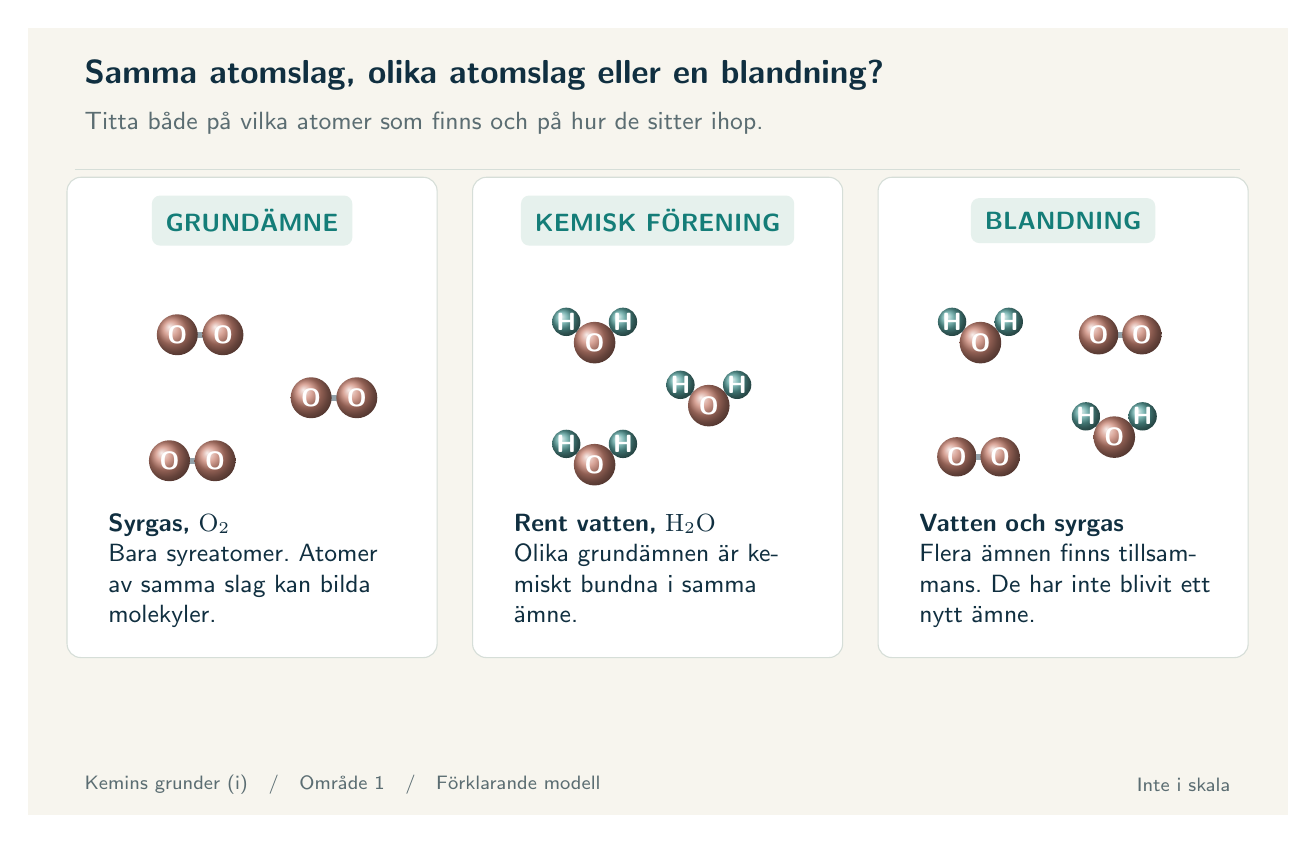
\begin{tikzpicture}[x=1cm,y=1cm]
\path[use as bounding box] (0,0) rectangle (16,10);
\fill[paper] (0,0) rectangle (16,10);
\node[head] at (.6,9.4){Samma atomslag, olika atomslag eller en blandning?};
\note{.6}{9.05}{14.8}{\textcolor{muted}{Titta både på vilka atomer som finns och på hur de sitter ihop.}}
\draw[line] (.6,8.2)--(15.4,8.2);

\foreach \x in {.5,5.65,10.8}{\panel{\x}{2}{4.7}{6.1}}
\node[badge] at (2.85,7.55){GRUNDÄMNE};\node[badge] at (8,7.55){KEMISK FÖRENING};\node[badge] at (13.15,7.55){BLANDNING};
\foreach \x/\y in {1.9/6.1,3.6/5.3,1.8/4.5}{\draw[navy!45,line width=2pt] (\x,\y)--++(.58,0);\atom{\x}{\y}{rust}{O}{.26}\atom{\x+.58}{\y}{rust}{O}{.26}}
\water{7.2}{6}{1.2}\water{8.65}{5.2}{1.2}\water{7.2}{4.45}{1.2}
\water{12.1}{6}{1.2}\water{13.8}{4.8}{1.2}
\draw[navy!45,line width=2pt] (13.6,6.1)--(14.15,6.1);\atom{13.6}{6.1}{rust}{O}{.25}\atom{14.15}{6.1}{rust}{O}{.25}
\draw[navy!45,line width=2pt] (11.8,4.55)--(12.35,4.55);\atom{11.8}{4.55}{rust}{O}{.25}\atom{12.35}{4.55}{rust}{O}{.25}
\note{.9}{3.95}{3.9}{\textbf{Syrgas, $\mathrm{O_2}$}\par Bara syreatomer. Atomer av samma slag kan bilda molekyler.}
\note{6.05}{3.95}{3.9}{\textbf{Rent vatten, $\mathrm{H_2O}$}\par Olika grundämnen är kemiskt bundna i samma ämne.}
\note{11.2}{3.95}{3.9}{\textbf{Vatten och syrgas}\par Flera ämnen finns tillsammans. De har inte blivit ett nytt ämne.}\node[anchor=west,text=muted,font=\scriptsize] at (.6,.38){Kemins grunder (i)\quad /\quad Område 1\quad /\quad Förklarande modell};
\node[anchor=east,text=muted,font=\scriptsize] at (15.4,.38){Inte i skala};
\end{tikzpicture}\end{document}
